\documentclass[a4paper]{article}\usepackage[]{graphicx}\usepackage[]{color}
%% maxwidth is the original width if it is less than linewidth
%% otherwise use linewidth (to make sure the graphics do not exceed the margin)
\makeatletter
\def\maxwidth{ %
  \ifdim\Gin@nat@width>\linewidth
    \linewidth
  \else
    \Gin@nat@width
  \fi
}
\makeatother

\definecolor{fgcolor}{rgb}{0.345, 0.345, 0.345}
\newcommand{\hlnum}[1]{\textcolor[rgb]{0.686,0.059,0.569}{#1}}%
\newcommand{\hlstr}[1]{\textcolor[rgb]{0.192,0.494,0.8}{#1}}%
\newcommand{\hlcom}[1]{\textcolor[rgb]{0.678,0.584,0.686}{\textit{#1}}}%
\newcommand{\hlopt}[1]{\textcolor[rgb]{0,0,0}{#1}}%
\newcommand{\hlstd}[1]{\textcolor[rgb]{0.345,0.345,0.345}{#1}}%
\newcommand{\hlkwa}[1]{\textcolor[rgb]{0.161,0.373,0.58}{\textbf{#1}}}%
\newcommand{\hlkwb}[1]{\textcolor[rgb]{0.69,0.353,0.396}{#1}}%
\newcommand{\hlkwc}[1]{\textcolor[rgb]{0.333,0.667,0.333}{#1}}%
\newcommand{\hlkwd}[1]{\textcolor[rgb]{0.737,0.353,0.396}{\textbf{#1}}}%
\let\hlipl\hlkwb

\usepackage{framed}
\makeatletter
\newenvironment{kframe}{%
 \def\at@end@of@kframe{}%
 \ifinner\ifhmode%
  \def\at@end@of@kframe{\end{minipage}}%
  \begin{minipage}{\columnwidth}%
 \fi\fi%
 \def\FrameCommand##1{\hskip\@totalleftmargin \hskip-\fboxsep
 \colorbox{shadecolor}{##1}\hskip-\fboxsep
     % There is no \\@totalrightmargin, so:
     \hskip-\linewidth \hskip-\@totalleftmargin \hskip\columnwidth}%
 \MakeFramed {\advance\hsize-\width
   \@totalleftmargin\z@ \linewidth\hsize
   \@setminipage}}%
 {\par\unskip\endMakeFramed%
 \at@end@of@kframe}
\makeatother

\definecolor{shadecolor}{rgb}{.97, .97, .97}
\definecolor{messagecolor}{rgb}{0, 0, 0}
\definecolor{warningcolor}{rgb}{1, 0, 1}
\definecolor{errorcolor}{rgb}{1, 0, 0}
\newenvironment{knitrout}{}{} % an empty environment to be redefined in TeX

\usepackage{alltt}

\usepackage[english]{babel}
\usepackage[utf8]{inputenc}
\usepackage{amsmath, amssymb, amsthm}
\usepackage{graphicx}
\usepackage[colorinlistoftodos]{todonotes}
\usepackage{float}
\usepackage[margin=0.75in]{geometry}

\newtheorem{thm}{Theorem}[section]
\newtheorem{defn}{Definition}[section]
\newtheorem{ex}{Example}[section]

\title{CIS 520 - Machine Learning Notes}
\author{Eric Oh - University of Pennsylvania}
\date{\today}
\IfFileExists{upquote.sty}{\usepackage{upquote}}{}
\begin{document}
\maketitle

\section{Local Learning}

The class of local learning methods seems less like learning and more like pure memorization - and in some ways it is. Main idea: given a new example $x$, find the most similar training example(s) and predict a similar output. We generally assume some measure of similarity or distance between examples and learn a \emph{local} method in a neighborhood of the new example. Consider the one dimensional regression problem:

\begin{figure}[H]
\centering
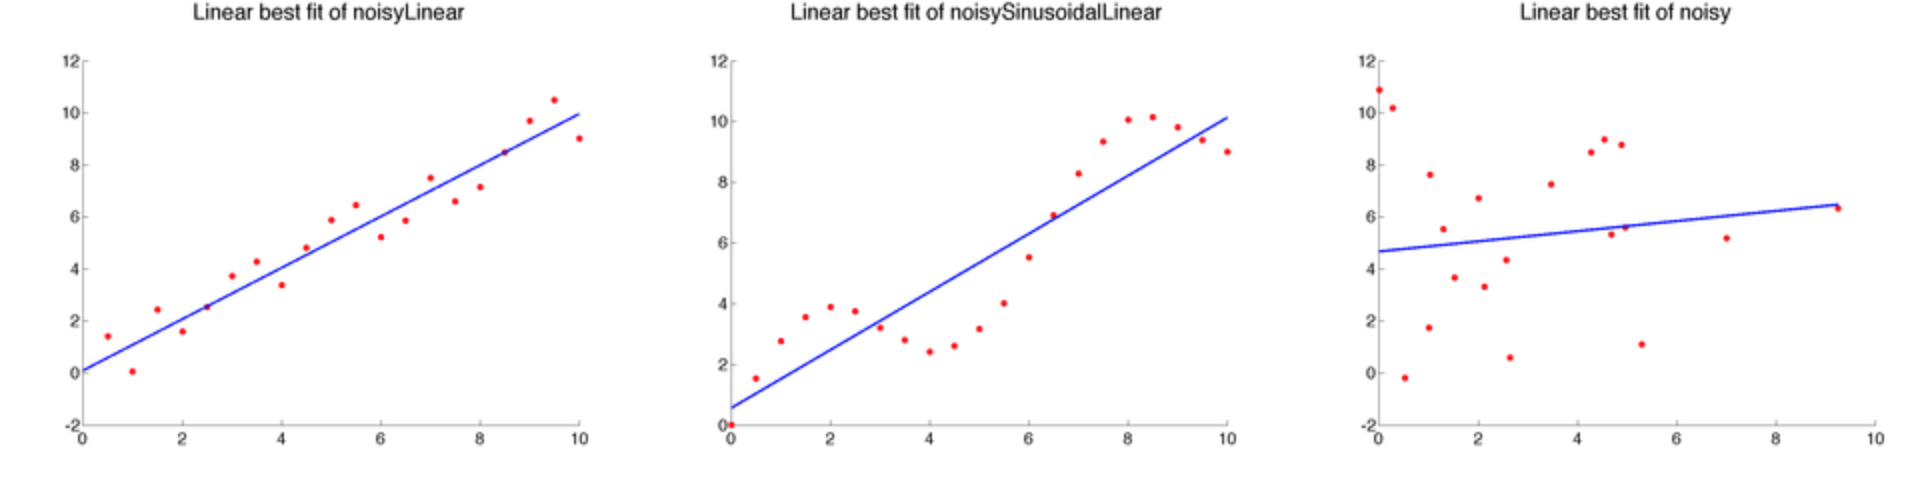
\includegraphics[width=6in]{badlinreg.png}
\caption{Clearly, linear model doesn't fit data well always}
\end{figure}

\subsection{Nearest Neighbor}

We could try adding higher-order polynomial terms or try a local method like nearest neighbors:

\begin{verbatim}
1 - Nearest Neighbor Algorithm 
  1. Given training data D={x_i,y_i}, distance function d(.,.), and input x
  2. Find j = arg min_i d(x,x_i) and return y_j
\end{verbatim}

Some examples of the above algorithm with $d(x,x_i)=|x-x_i|$ as x varies:

\begin{figure}[H]
\centering
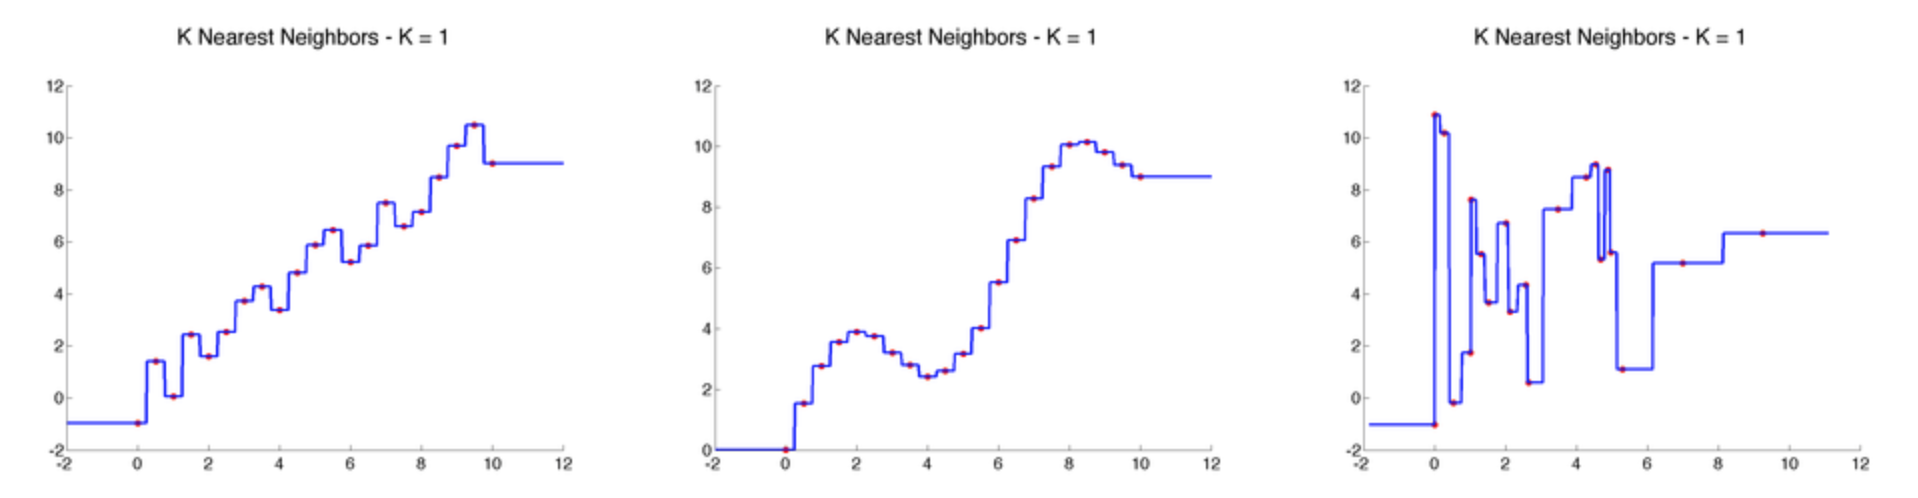
\includegraphics[width=6in]{1NN.png}
\end{figure}

Generally, we use some arbitrary distance function to define nearest neighbor. Some common choices are the $L_1$, $L_2$, or the $L_{\infty}$ norms. 

\begin{defn}
\textbf{Norm} - for all $a \in \mathbb{R}$ and all $u,v \in V$,
\begin{itemize}
\item $L_p(av) = |a|L_p(v)$
\item $L_p(u+v) \leq L_p(u) + L_p(v)$ - \emph{triangle inequality or subadditivity}
\item If $L_p(v)=0$ then v is the zero vector
\end{itemize}
\end{defn}

\begin{ex}
$L_p$ norm : $\left(\sum_{j}|x_j|^p\right)^{\frac{1}{p}}$
\end{ex}

\begin{defn}
\textbf{$L_0$ pseudo-norm} : $|x|_0$ = number of $x_j \neq 0$ 
\end{defn}

The contours of the most common distance measures are below.

\begin{figure}[H]
\centering
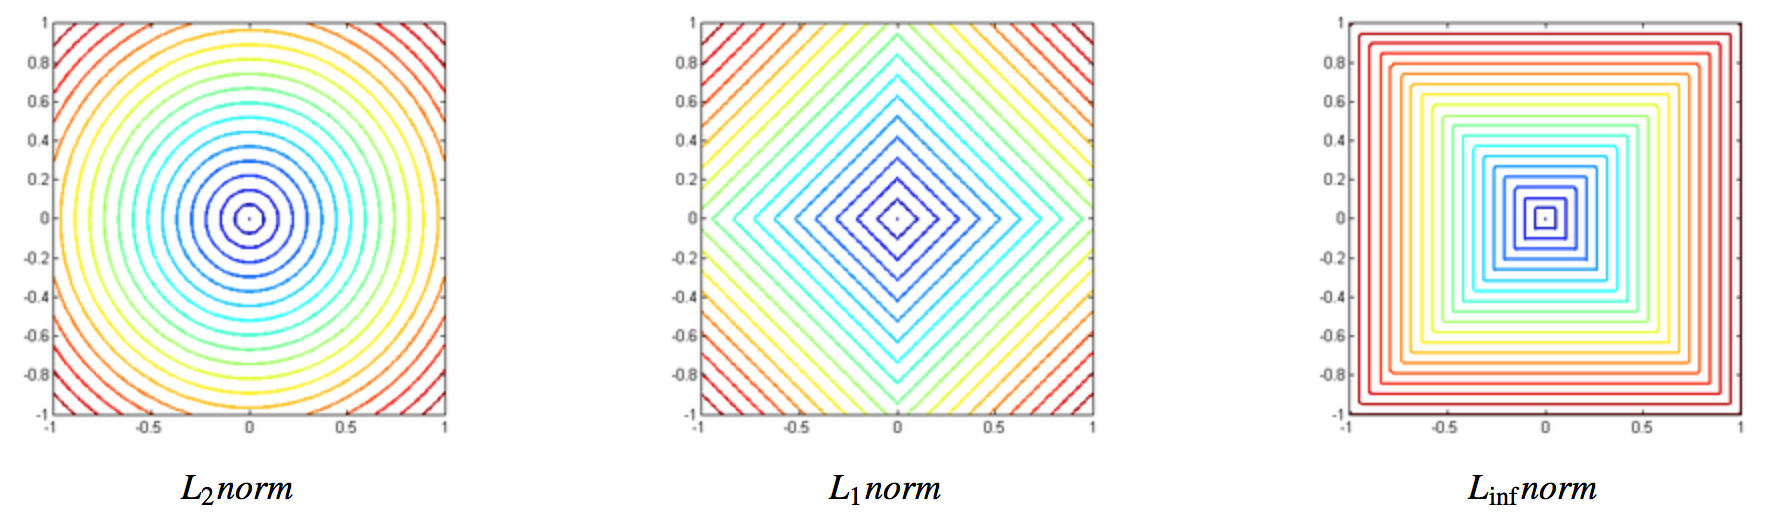
\includegraphics[width=6in]{norm_contour.png}
\end{figure}

Note that for the $L_p$ norm, p must be at least 1. $L_p$ norms with $p<1$ result in \textbf{concave} contours - NOT GOOD. So how do norms delate explicitly to distances?

\begin{equation*}
d_p(x,y) = |x-y|_p
\end{equation*}

Note that norms are \textbf{SCALE-INVARIANT}. Thus, if $x$ is a vector of non-negative terms, then 
\begin{align*}
\sum_i x_i \hspace{0.5in} \text{and} \hspace{0.5in} \sum_i ix_i
\end{align*}

are both norms. \\

1-Nearest Neighbor is one of the simplest examples of a \textbf{non-parametric} method (ie. model structure determined by the training data). Non-parametric models are much more flexible and expressive than parametric models, and thus \textbf{overfitting} can be a big concern. One nice property of NP models is that since the complexity increases as the data increases, with enough data, NP models can model nearly anything and achieve close to zero bias for any distribution (ie. consistent..sort of). A huge problem with this, however, is that for any finite sample size there will likely be huge variance (ie. overfitting). \\

One way to reduce the variance is local averaging : instead of just one neighbor, find K and average their predictions. 

\begin{verbatim}
K-Nearest Neighbors Algorithm
  1. Given training data D={x_i,y_i}, distance function d(.,.), and input x
  2. Find {j_1,...,j_K} closest examples wrt d(x,.)
      a. (Regression) if y \in \mathbb{R}, return average of y_{j_k}
      b. (Classification) if y is 1 or -1, return majority
\end{verbatim}

\begin{figure}[H]
\centering
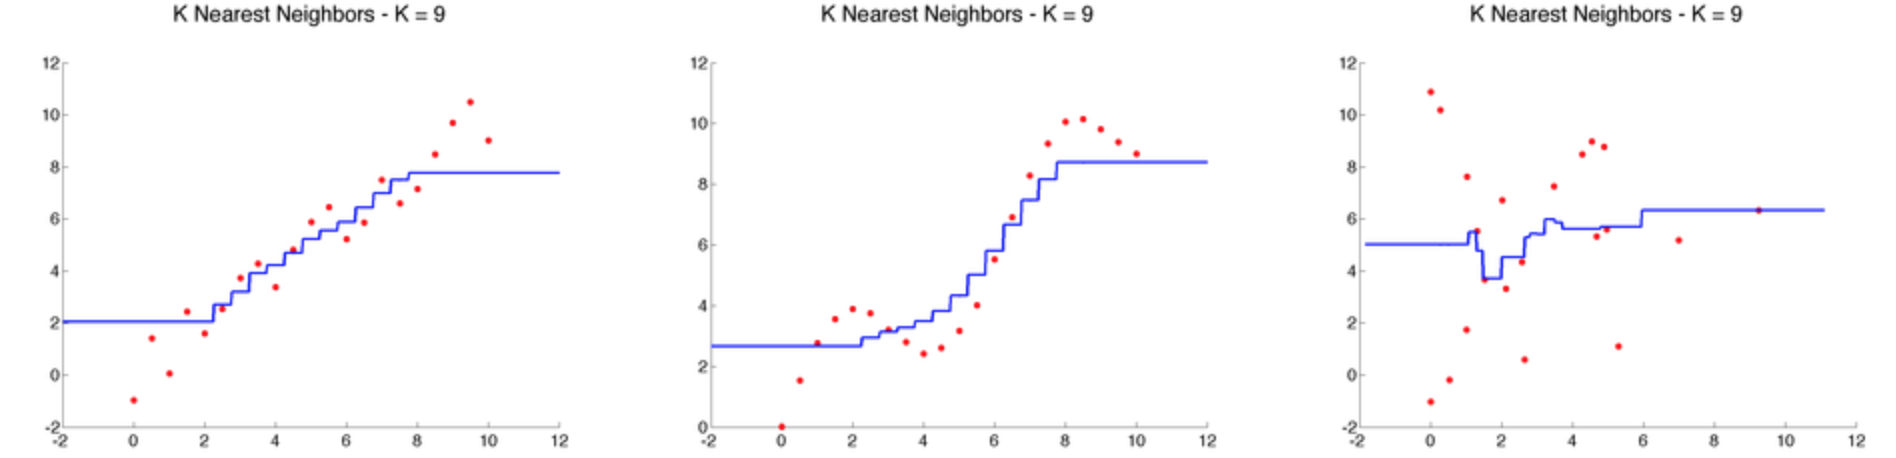
\includegraphics[width=6in]{9NN.png}
\caption{9 nearest neighbors - smoother prediction but edges still sketchy}
\end{figure}

\subsection{Kernel Regression}

Two main shortcomings of K-NN method:
\begin{enumerate}
\item All neighbors receive equal weight
\item Number of neighbors chosen globally
\end{enumerate}

Kernel regression address these issues by \emph{using all neighbors} but with different weights (ie. closer neighbors receiving higher weights and vice versa). Weighting function is a \textbf{kernel} and it measures similarity (as opposed to distance) between examples. Can convert from a distance d(.,.) to kernel K(.,.) easily - most common way is via Gaussian kernel (ignoring normalizing constants):

\begin{equation*}
K(x,x_i) = \exp\left(\frac{-d^2(x,x_i)}{h}\right)
\end{equation*}

Kernel Regression/Classification Algorithm
\begin{enumerate}
\item Given training data $D={x_i,y_i}$, Kernel function K(.,.), and input x
\begin{itemize}
\item (Regression) if $y \in \mathbb{R}$, return weighted average: $\sum_i y_i \frac{K(x,x_i)}{\sum_j K(x,x_j)}$
\item (Classification) if $y \in \pm 1$, return weighted majority: $\mbox{sgn}\left(\sum_i y_iK(x,x_i)\right)$
\end{itemize}
\end{enumerate}

One of the keys kernel regression is $h$, the \textbf{bandwidth}, which determines how quickly the influence of neighbors falls off with distance. The following shows the effect of increasing levels of $h$. 

\begin{figure}[H]
\centering
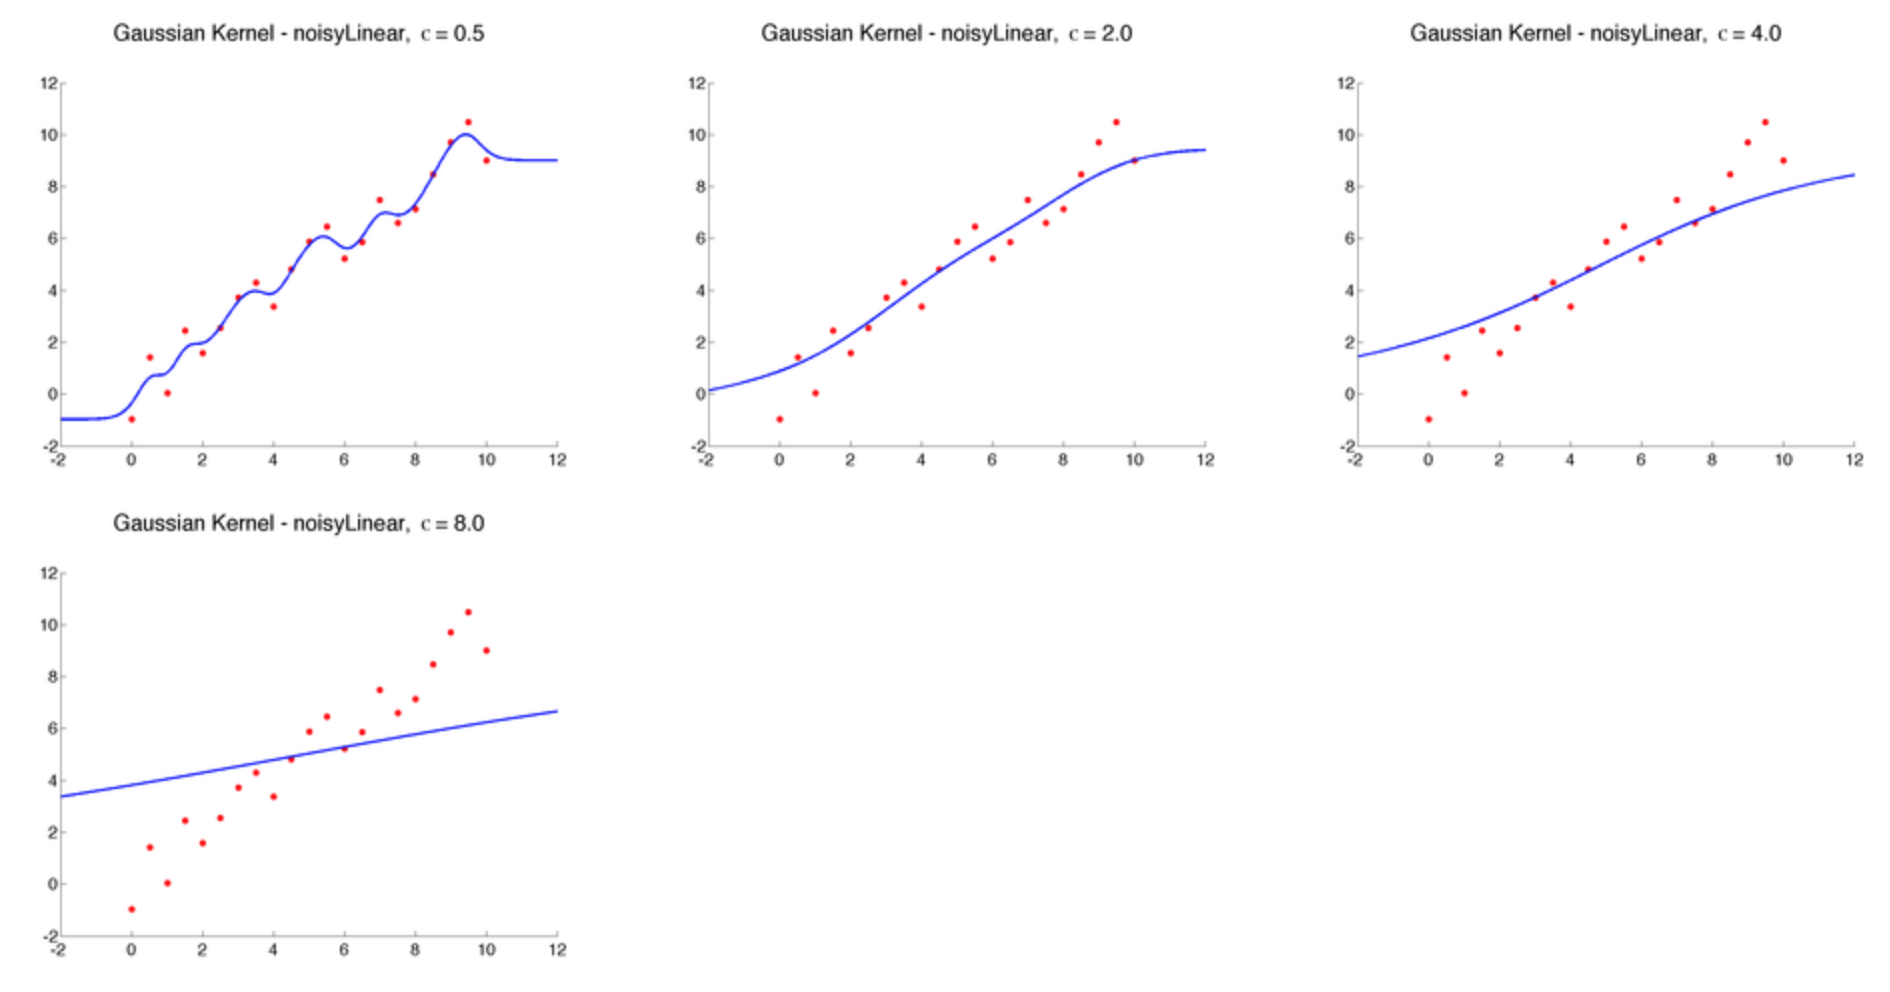
\includegraphics[width=6in]{kernel_reg.png}
\end{figure}

As $h \rightarrow \infty$, all the neighbors weight the same and the prediction is the global average. \\
As $h \rightarrow 0$, prediction tends to 1-NN. \\
Clearly choosing the ``right" $h$ is very important - in practice, usually use \textbf{cross-validation} to pick.

\section{Decision Trees}

\begin{itemize}
\item Gives nice interpretable output but each split uses exponentially less data (observations)
\item How do we decide which features to split on? How to define importance? Need definition of information
\end{itemize}

\subsection{Entropy}
Suppose X can have one of $m$ values, $V_1,\ldots,V_m$, with $P(X=V_i)=p_i$. Entropy is the smallest possible number of bits, on average, per symbol, needed to transmit a stream of symbols drawn from X's distribution. 

\begin{defn}
Entropy : $H(X) = -\sum_{j=1}^m p_j \log_2 p_j$
\end{defn}

\begin{itemize}
\item High entropy : X is from uniform (boring) distribution. Values sampled from it would be all over the place.
\item Low entropy : X is from varied (valleys and peaks) distribution. Values sampled from it would be more predictable (from the peaks).
\end{itemize}

\textbf{Entropy} is the expected value of the information content (surprise) of the message $\log_2 p_j$. Range of entropy is from 0 to $\infty$. 

\begin{ex}
\begin{enumerate}
\item If an event is certain, entropy is 0
\item If two events are equally likely, entropy is 1 $(-\left(-0.5 * \log(0.5) + -0.5 * \log(0.5)\right)$
\end{enumerate}
\end{ex}

\begin{defn}
Specific Conditional Entropy : $H(Y|X=v)$, the entropy of Y among only those records in which X has value v.
\end{defn}

\begin{figure}[H]
\centering
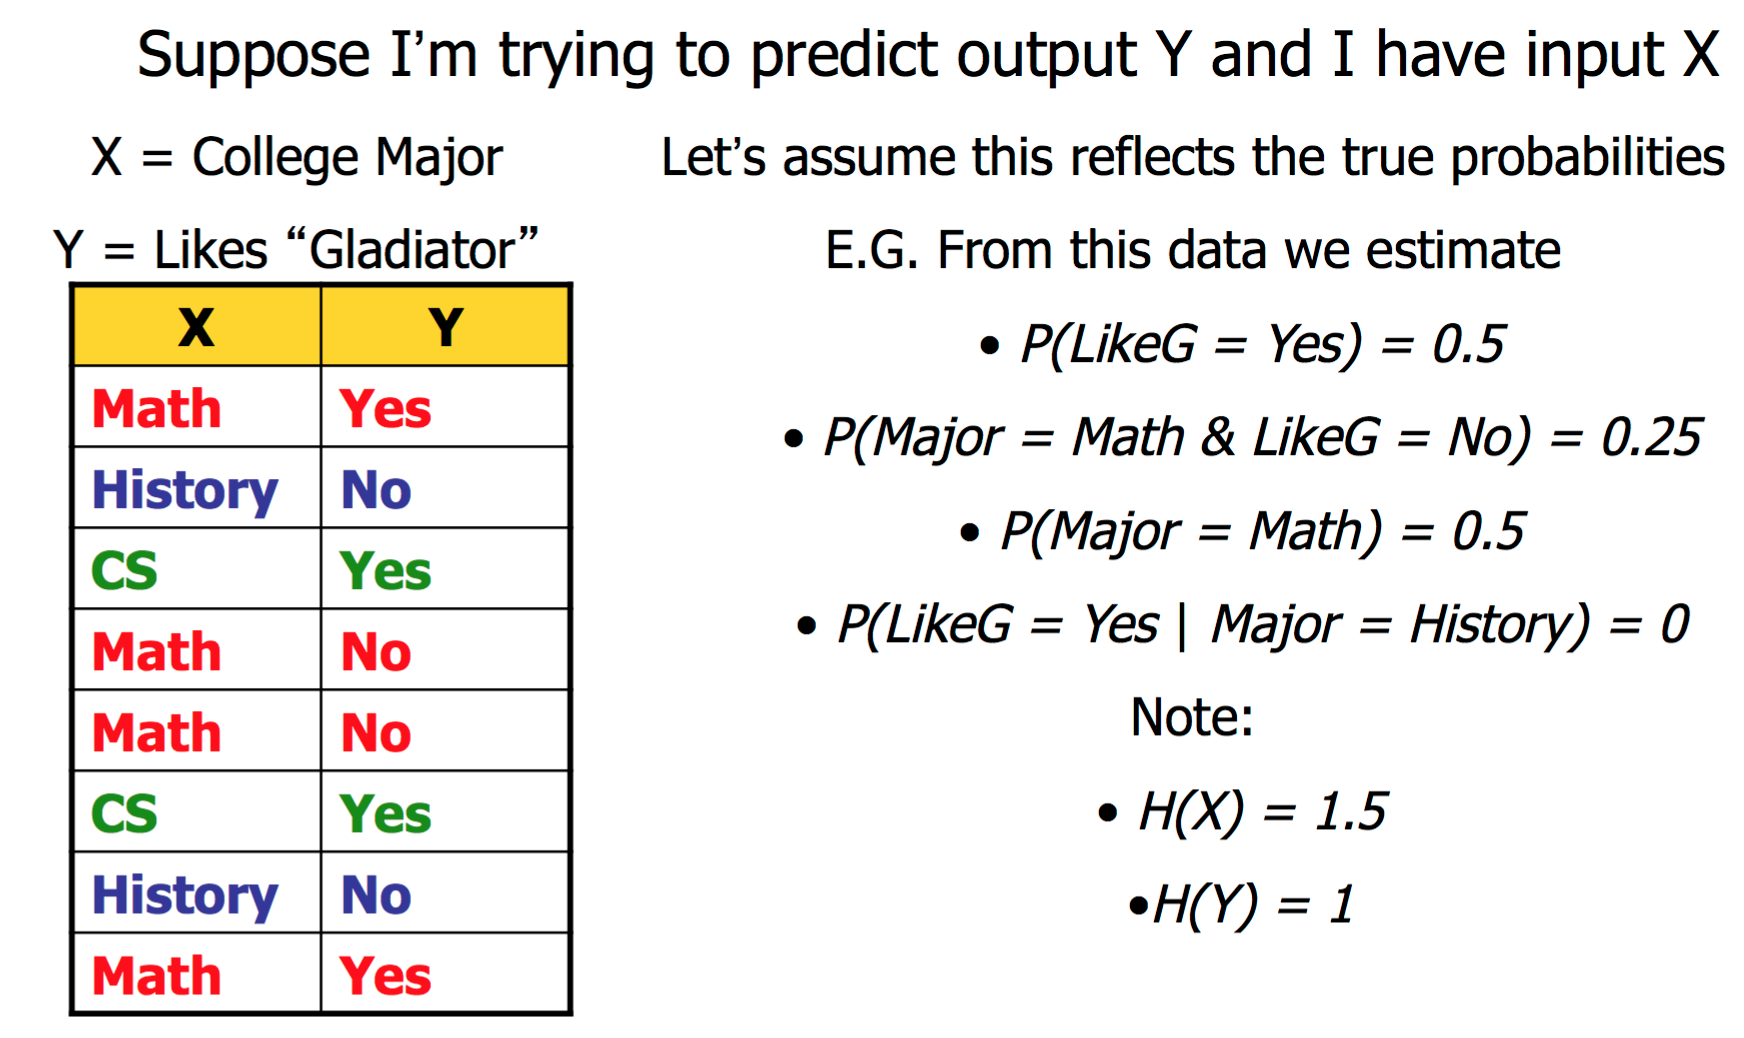
\includegraphics[width=6in]{cond_ent_ex.png}
\end{figure}

\begin{defn}
Conditional Entropy : $H(Y|X)=\sum_j P(X=v_j)H(Y|X=v_j)$, the average specific conditional entropy of Y 
\end{defn}


\begin{figure}[H]
\centering
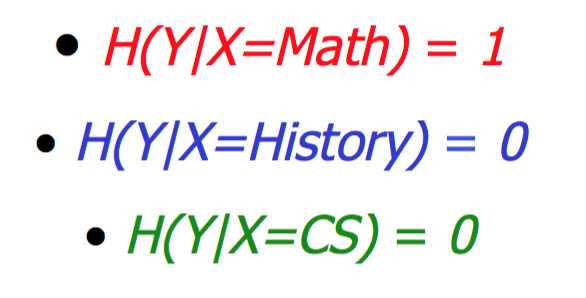
\includegraphics[width=1.5in]{specific_condent.png}
\end{figure}

\begin{defn}
Information Gain : $IG(Y|X) = H(Y)-H(Y|X)$, how many bits on average would it save me in transmitting Y if both ends of the line knew X? 
\end{defn}

\begin{ex}
Suppose, \\
$H(Y)=1, H(Y|X)=0.5$. Then $IG(Y|X) = 1-0.5=0.5$, and knowing X gives gain of 0.5 information (unit is bits). 
\end{ex}

Note: range of IG is from 0 to $\infty$. If Y and X are independet, then $IG=0$. \\
In general, features with more options (more categories) have more possible information gain than binary features. \\
\\
\textbf{Key to Decision Trees}: How do we prevent overfitting? How we know when to stop splitting?! Number of leaves grows exponentially


\section{MLE}

Self-explanatory. 

\subsection{Learning Guarantees}

The following bound will be useful (based on Hoeffding inequality): 

\begin{thm}
$P(|\hat{\theta}_{MLE}-\theta| \geq \epsilon) \leq 2e^{-2n\epsilon^2}$
\end{thm}

In other words, MLE deviates from true parameter exponentially with $n$. 

\section{MAP (maximum a posteriori)}

Bayes rule gives 

\begin{equation*}
P(\theta|D) = \frac{P(D|\theta)P(\theta)}{P(D)}
\end{equation*}

\begin{defn}
$\hat{\theta}_{MAP} = \mbox{arg max}_{\theta} P(\theta|D) = \mbox{arg max}_{\theta} \log(P(D|\theta)) + \log(P(\theta)) $
\end{defn}

Note: the $\log(P(\theta))$ acts as a regularizer for the log likelihood for MAP estimation. \\
Note: as $n \rightarrow \infty$, the prior's effect vanishes and we recover the MLE.\\
Note: MAP is the simplest Bayesian approach to parameter estimation - sets estimate equal to mode of posterior distribution $P(\theta|D)$. There is more information in the posterior such as the mean and variance of the distribution. 


\section{Regression}

\subsection{Ridge Regression}

If we have too many features compared to data points, we want to do some regularization. Ridge regression does this with an $L_2$ penalization. For instance
\begin{equation*} W = (X^T X)^{-1} X^T Y \end{equation*}
wouldn't work with too many features (ie. $(X^T X)$ not invertible). Thus we minimize
\begin{equation*} \lVert y-X\beta \rVert_2 + \lambda \lVert \beta \rVert_2 \end{equation*}
which eseentially finds $W=(X^T X + \lambda I)^{-1} X^T Y$. The addition of the penalty makes the matrix positive semi definite and invertible. 

\section{Classification}

Goal: Learn to predict a categorical outcome from input and minimize expected classification error:
\begin{equation*}
E{(x,y)}[I(h(x)\neq y)]
\end{equation*}

If we had binary data (0's and 1's), we could fit linear regression and just predict everything $>0.5$ to be 1 and everything $<0.5$ to 0. We \textbf{CAN} fit linear regression to binary data, but this is bad!! This gives probabilities below 0 and above 1!! \\
\\
Make a transformation! Most common one is \textbf{logit} function:
\begin{equation*}
f(s) = \frac{1}{1+e^{-s}}
\end{equation*}

\subsection{Generative v. Discriminative Approaches}
One of the main distinctions between classification algorithms is the distinction between Generative and Discriminative. Essentially, 
\begin{itemize}
\item Generative classifiers model $P(x,y)$
\item Discriminative classifiers model $P(y|x)$
\end{itemize}

\textbf{Generative Approach}
Estimate $\hat{P(x,y)}$ from training data (ie. MLE or MAP) and then produce classifier:
\begin{align*}
h(x) = \text{argmax}_y \hat{P(y|x)} = \text{argmax}_y \frac{\hat{P(x,y)}}{\sum_{y'}\hat{P(x,y)}}
\end{align*}

For binary classification, this reduces to 
$h(x) = \left\{\begin{array}{lr}
1, & \text{if } \hat{P(x,1)} > \hat{P(x,-1)} \\
0, & \text{otherwise } \\
\end{array}\right\}$

If we are \textbf{very} lucky and learn a perfect model for $P(x,y)$, then we are \textbf{Bayes optimal}. But usually never happens. One example of a generative model is \textbf{Naive Bayes}. \\
\\
\textbf{Discriminative Approach}
Joint distribution $P(x,y)$ is hard to model, so focuses on $P(y|x)$. 
\begin{itemize}
\item Logistic regression models $P(y|x)$ as logit-linear and then estimates params using MLE or MAP 
\item SVM and boosting learn a function $h(x)$ that minimizes expected classification error 
\end{itemize}

\subsection{Logistic Regression}

Thus we obtain something like (for Y=1 and Y=-1)
\begin{align*}
P(Y=1|x,w) &= \frac{1}{1+\exp(-w^Tx)} = \frac{1}{1+\exp(-yw^Tx)} \\
P(Y=-1|x,w) &= 1-P(Y=1|x,w) = \frac{\exp(-w^Tx)}{1+\exp(-w^Tx)} = \frac{1}{1+\exp(-yw^Tx)} \\
\end{align*}

Log-likelihood for logistic regression can be written
\begin{align*}
\log(P(D_y|D_x,w)) = \log\left(\prod_i \frac{1}{1+\exp(-y_i w^T x_i)}\right) = -\sum_i \log(1+\exp(-y_i w^T x_i))
\end{align*}

Since log-likelihood for logistic regression is concave downwards (or convex upwards), can solve using \textbf{gradient ascent}! \\
\\
Start at some initial point $w^0=0$ and climb up in the steepest direction defined by the gradient of our objective function. The gradient ascent update is
\begin{align*}
w^{t+1} = w^t + \nu_t \triangledown_w l(w)
\end{align*}
where $\nu_t$ is the update rate and $\triangledown_w l(w)=\sum_i y_i x_i (1-P(y_i|x_i,w_i))$ \\
\\
\textbf{Why is the decision bounary linear?}\\
Consider the condition that holds at the boundary:
\begin{align*}
P(Y=1|x,w)=P(Y=-1|x,w) \Rightarrow \frac{1}{1+\exp(-w^T x)} = \frac{\exp(-w^T x)}{1+\exp(-w^T x)} \Rightarrow w^Tx =0 
\end{align*}

Solving that system gives a line!!\\
\\
\textbf{Computing MAP}\\
We can assume a prior distribution on the parameters $w$ that we are trying to estimate. Assume 
\begin{equation*} w_j \sim \text{N}(0,\lambda^2) \rightarrow P(w)=\prod_j \frac{1}{\lambda\sqrt{2\pi}}\exp\left(\frac{-w_j^2}{2\lambda^2}\right)\end{equation*}
giving an objective function of
\begin{align*}
\text{argmax}_w \log(P(w|D,\lambda)) = \text{argmax}_w (l(w) + P(w|\lambda)) = \text{argmax}_w \left(l(w) + \frac{1}{2\lambda^2}w^T w\right)
\end{align*}
We can solve for $w$ similarly using gradient ascent. Note that the effect of the prior is to \textbf{penalize} large values of $w$. 

Can also do the same as above with multinomial outcomes!
\begin{align*}
P(Y=k|x,w) = \frac{\exp(w_k^T x)}{1+\sum_{k'=1}^{K-1} \exp(w_{k'}^T x)} \hspace{0.3in} k=1,\ldots,K
\end{align*}

\subsection{Naive Bayes}

Naive Bayes classifier is an example of a \textbf{generative} model : we model $P(x,y)=P(y)P(x|y)$ where
\begin{itemize}
\item $P(y)$ : class prior
\item $P(x|y)$ : class model
\end{itemize}

We estimate them separately as $\hat{P(y)}$ and $\hat{P(x|y)}$. Note: the class prior is different than the parameter prior classic Bayesian analysis. We then use our estimates to output a classifier using Bayes rules:

\begin{align*}
h(x) = \text{argmax}_y \hat{P(y|x)}  = \text{argmax}_y \frac{\hat{P(y)}\hat{P(x|y)}}{\sum_y \hat{P(y)}\hat{P(x|y)}} \propto \text{argmax}_y \hat{P(y)}\hat{P(x|y)}
\end{align*}

\text{In English}: Classify a new instance $x$ based on a tuple of attribute values $x=(x_1,\ldots,x_n)$ into one of the classes $y_j \in Y$. \\
\\

\textbf{Estimating $P(y)$} : Can be estimated from the frequency of classes in the training examples\\
\\
\textbf{Estimating $P(x|y)$} : The \emph{Naive Bayes assumption} is that $P(x|y) = \prod_i \hat{P(x_i|y)}$ (Conditional independence) \\
\\

If we assume both $Y$ and $X$ are discrete, can do (MLE estimation)
\begin{align*}
\hat{P(y)} = \frac{N(y=y_j)}{N} \hspace{0.5in} \hat{P(x_i|y)} = \frac{N(x_i=x_j,y=y_j)}{N(y=y_j)}
\end{align*}

Note: If $Y$ and/or $X$ are continuous, we can pick some model for the distribution (ie. Gaussian). \\
\\

Problem with MLE though is that if we see no training examples for some class, we have 0 probabilities! To deal with this, we can smooth the probabilities to avoid overfitting. 
\begin{align*}
\hat{P(x_i|y)} = \frac{N(x_i=x_j,y=y_j)+mP_{i,k}}{N(y=y_j)+m}
\end{align*}

This is sort of like \textbf{empirical bayes} where our prior includes information on probabilities in the entire sample?  \\
\\
Note for implementation: DO NOT MULTIPLY PROBABILITIES. THIS LEADS TO UNDERFLOW. INSTEAD ADD LOG PROBABILITIES.


\subsection{MAP}

To take care of the 0 probability problem with MLE, just add a prior to each $x_j$ (Ie. for counts of words in topic documents, adding $\text{Beta}(0.5,0.5)$ is a Jeffrey's prior, adding $\text{Beta}(1,1)$ is Laplace smoothing). BUT THIS KIND OF SUCKS. We know ``the" is more common, so instead we could use an \textbf{empirical bayes} thing where the prior is proportional to how often we see in data. 


\subsection{Naive Bayes vs Logistic Regression}

\begin{figure}[H]
\centering
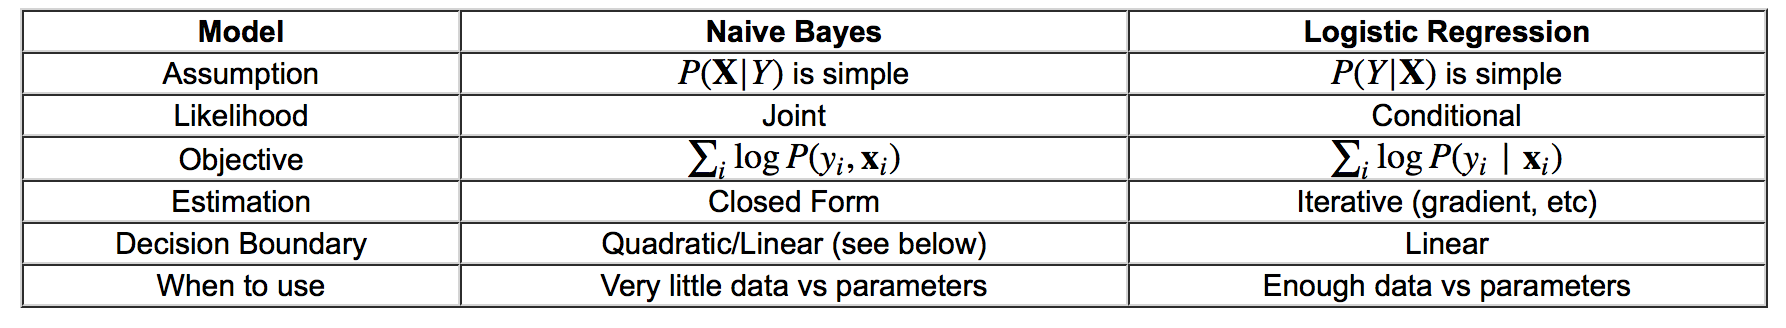
\includegraphics[width=5in]{NBvsLogit.png}
\end{figure}

\begin{itemize}
\item If we only care about probabilities, probably better to use logisitic regression.  
\item If we only care about which class is most likely, might be better to use Naive Bayes. 
\end{itemize}

If variance of the classes are wildly different, there can be a non-linear boundary for Naive Bayes. If we assume that $P(X_j|Y)$ is Gaussian and Y is binary and $P(X_j|Y)$ have same variance for both classes, then can show that it is equivalent to logistic regression. 

\section{Basis Functions}
We can still learn difficult, non-separable datasets by transforming the inputs using \textbf{basis functions}. Can create new, good features. Consider the XOR dataset

\begin{figure}[H]
\centering
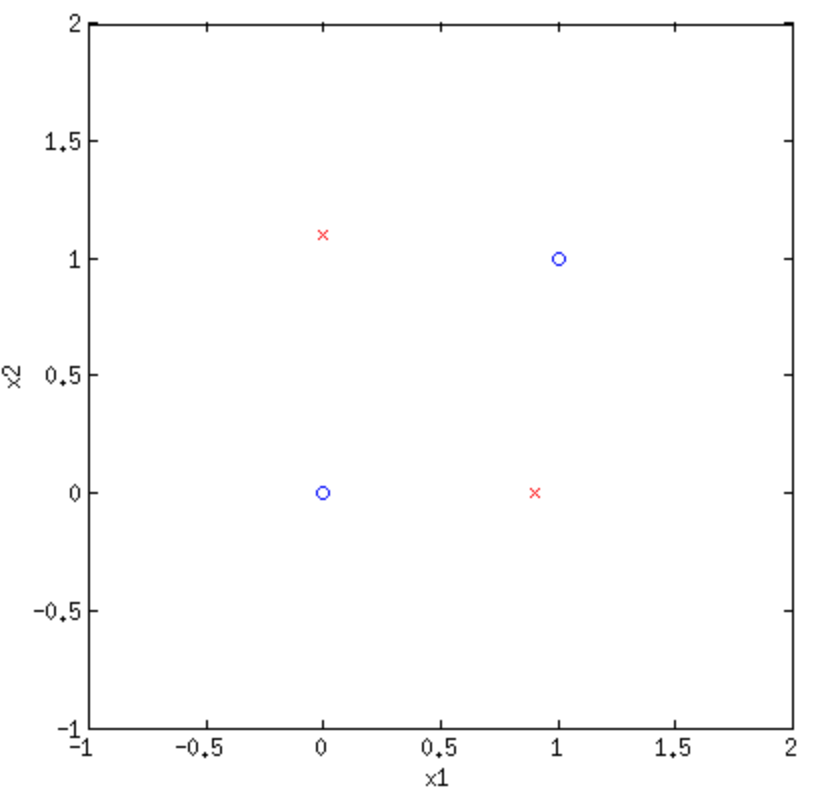
\includegraphics[width=2.5in]{xor_data.png}
\end{figure}

One basis that works quite well is \textbf{radial basis functions (RBF)}. 
\begin{defn}
\textbf{RBF} is a real-valued function whose values depends only on the distance between the point and some ``center" c : 
\begin{equation*} \phi(x,c) = \phi(\lVert x-c \rVert) \end{equation*}
\end{defn}

Common functions include the Gaussian and various polynomials. Often need to cross-validate to pick the best hyperparameters. 

\begin{ex}
For Gaussian basis, $\exp\left(\frac{(x-\mu_K)^2}{c}\right)$, need to pick best number of centers $K$ and the width $c$ for each.
\end{ex} 

To find the locations of the centers, standard RBF will use K means clustering to find the K clusters and put the $K$ centers there.  \\
\\
Note: RBF's are \textbf{NOT SCALE INVARIANT}. Gaussian basis assumes that all features are of equal importance. Any time we use some distance (ie. in a Kernel), there is this implicit assumption. 


\section{Overfitting and Regularization}

Overfitting happens when a model learns to describe noise in addition to the real dependencies between input and output. In terms of bias/variance decomposition, a very complex model can have small error on any dataset (training examples) but large error on new examples (test data) due to the variance being too high. 

\begin{ex}
\begin{itemize}
\item For RBFs, number of centers and width of gaussians measures complexity (increase number of centers and make width smaller to increase complexity)
\item $\lambda$ in ridge regression measures complexity $\left(\frac{1}{\lambda}\right)$
\item $K$ in KNN measures complexity $\left(\frac{1}{K}\right)$
\item Depth of tree in Decision Trees is one way to measure complexity 
\end{itemize}
\end{ex}

\begin{figure}[H]
\centering
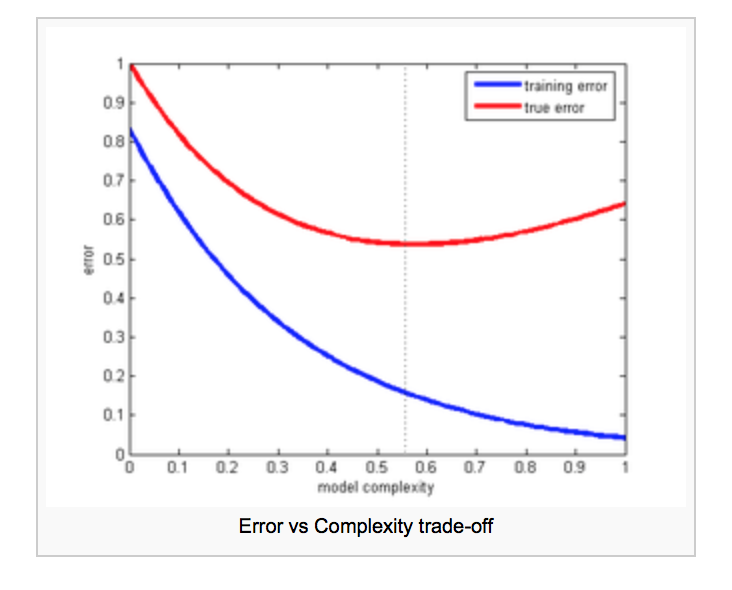
\includegraphics[width=3in]{overfit.png}
\end{figure}

\subsection{Adjusting complexity penalty using \textbf{Cross-Validation}}

ASSUMES I.I.D DATA. HAVE TO BE VERY CAREFUL FOR TIME SERIES.

\begin{defn}
\textbf{Leave one out CV (LOOCV)} : For each complexity setting, learn a classifer on \emph{all the training data except one example} and evaluate its error on the remaining example. Requires building n models....very slow! Only really used for datasets with less than 100 examples. 
\end{defn}

\textbf{Leave one out Error}:
\begin{align*}
\frac{1}{n} \sum_i I(h(x_i;D_{-1})\neq y_i)
\end{align*}
where $D_{-1}$ is the dataset minus the $i^{th}$ example and $h(x_i;D_{-1})$ is the classifier trained on that dataset. 

\begin{defn}
\textbf{K-fold CV} : Split the data into K subsets or folds (usually $K=10$) $D_1,\ldots,D_k$ and leave out each fold in turn for validation. 
\end{defn}

\textbf{K-fold Validation Error}:
\begin{align*}
\frac{1}{n}\sum_{k=1}^K \sum_{i \in D_k} I(h(x_i;D-D_k)\neq y_i)
\end{align*}
where $D-D_k$ is the dataset minus the $k^{th}$ fold and $h(x_i;D-D_k)$ is the classifier trained on that dataset. \\
\\
Note, often in industry, separating data into the development and validation sets is time dependent. We want to predict home prices/ stock prices/ etc. in the \textbf{FUTURE}. So we might train on data from 1996-2016 and then get validation error on 2017 data. (can't just take a simple random sample). \\
\\
If we have HUGE data (ie. Google, Facebook), can probably just split data 50-50 to train and test. 

\subsection{Bias/Variance Decomposition}

Can show that $\text{error} = E[(y-\hat{y})^2] = \text{Bias}(\hat{y})^2 + \text{Var}(\hat{y}) + \sigma^2 (noise)$.


\section{Regression Penalties and Priors}

\textbf{Review}: \\
\begin{itemize}
\item Given a set of observations with labels y
\item Generate features, $x$, for each observation (hardest, longest part)
\item Learn a regression model to predict y, $y=\beta x$ ; most of the $\beta$ are 0 though!!
\end{itemize}

\textbf{Two Interpretations of regression}: \\
\begin{enumerate}
\item Minimize (penalized) squared error
\item Maximize likelihood 
\end{enumerate}

Note: OLS (MLE) minimzes bias (doesn't care about overfitting). Ridge regression (or MAP) minimzes bias AND variance (penalizes non-important features). \\
\\
\textbf{Different Norms, different penalties}: \\
Minimize penalized error: $\lVert y-\beta x \rVert^2_2 + \lambda f(\beta)$
\begin{itemize}
\item $\lVert \beta \rVert_2 $ - $L_2$ makes all the $\beta_j$ a little smaller (RIDGE)
\item $\lVert \beta \rVert_1$ - $L_1$ drives some $\beta_j$ to 0 (LASSO or LARS)
\item $\lVert \beta \rvert_0$ - $L_0$ counts number of nonzero $\beta_j$ - ``stepwise regression"
\end{itemize}

all of the above encourage $\beta_j$ to be smaller, ie. shrink $\beta$. Bigger $\lambda$ gives more shrinkage!! $L_2$ and $L_1$ are nice because they are convex!! Can also do the \textbf{elastic net}:
\begin{align*}
\text{argmin}_{\beta} \lVert y - \beta x\rVert^2_2 + \lambda_1 \lVert \beta \rVert_1 + \lambda_2 \lVert \beta \rVert_2
\end{align*}

\subsection{Feature selection for regression}

Goal: minimize error for a test set \\
Approximation: minimize a penalized training set error \\
Note: always better to get approximation to correct loss function than get exact answer to wrong loss function!! \\

\textbf{Different regularization priors}
\begin{itemize}
\item $L_2$ corresponds to Gaussian prior: $p(\beta) = \exp\left(-\frac{\lVert \beta \rVert_2}{\sigma^2}\right)$ - not scale invariant?
\item $L_1$ corresponds to Laplace prior: $p(\beta) = \exp\left(-\frac{\lVert \beta \rVert_1}{\sigma^2}\right)$ - not scale invariant like OLS
\item $L_0$ corresponds to Spike and Slab, assumes some are 0?
\end{itemize}

\textbf{Solving regularization penalties}:
\begin{itemize}
\item $L_2$ - $\beta = (X^T X + \lambda I)^{-1} X^T y$
\item $L_1$ - convex optimization, gradient descent
\item $L_0$ - search (stepwise or streamwise)
\end{itemize}

\textbf{Properties}:
\begin{itemize}
\item $L_0$ norm most strongly encourages weights to be set to 0. 
\item $L_1$ and $L_0$ can handle exponentially more features than observations ; $L_2$ cannot
\item $L_2$:all $\beta$ shrink by constant factor
\item $L_1$:all $\beta$ shrink by constant amount (if $\beta$ lower than amount shrunk, then goes to 0. Determined by $\lambda$). Can be not great because to make a lot of features 0, must shrink all features by A LOT. (Does shrinkage and zeroing in ``one" step).
\item $L_0$ throws out all the non important features, leaves others?
\end{itemize}

If $x$'s have been standardized, can visualize the shrinkage:
\begin{figure}[H]
\centering
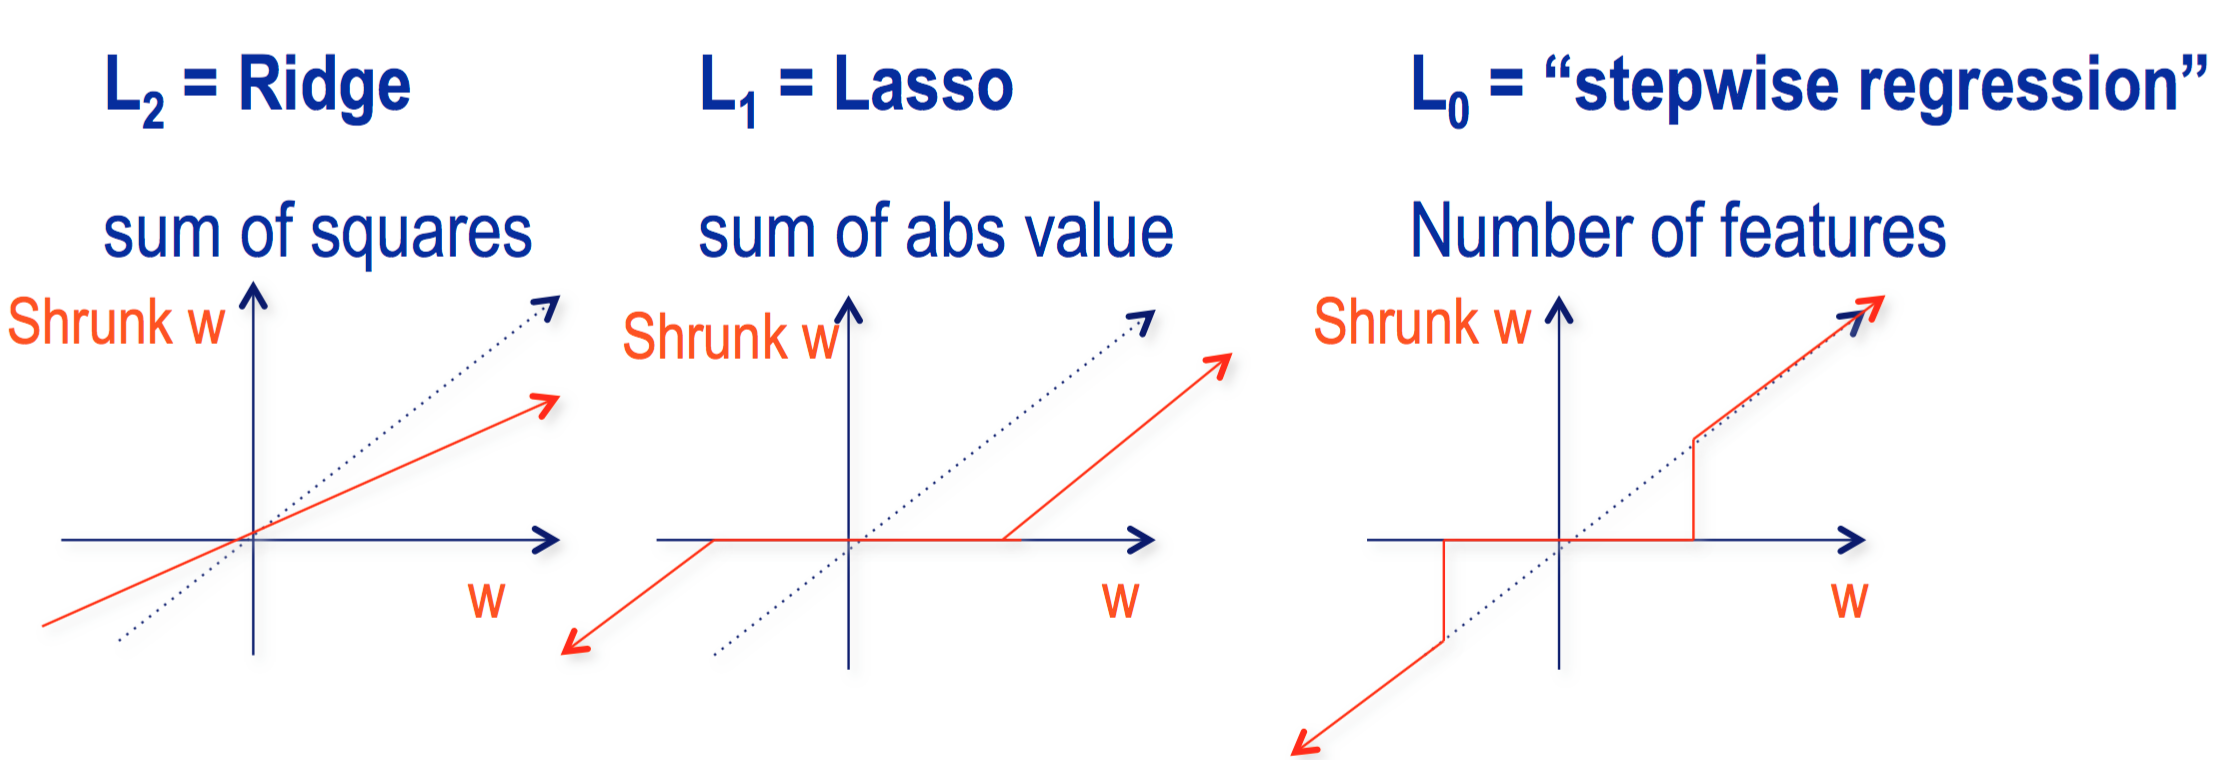
\includegraphics[width=5in]{regular_penalty.png}
\end{figure}


\subsection{Streamwise Regression}

\begin{enumerate}
\item Initialize :
\begin{itemize}
\item $\text{model} = \{\}$, $Err_0 = \sum_i (y_i-0)^2 + 0$
\end{itemize}

\item For each feature $x_j$:
\begin{itemize}
\item Try adding feature $x_j$ to the model
\item \textbf{if} $Err = \sum_i (y_i -\sum_j \beta_j x_{ij})^2 + \lambda \lVert \beta \rVert_0 < Err_{j-1}$, then accept new model and set $Err_j = Err$.
\item \textbf{else} Keep old model and set $Err_j = Err_{j-1}$
\end{itemize}
\end{enumerate}

The above algorithm is \textbf{extremely} greedy!! It is also biased to which features we try first...not great. 

\subsection{Stepwise Regression}

\begin{enumerate}
\item Initialize :
\begin{itemize}
\item $\text{model} = \{\}$, $Err_0 = \sum_i (y_i-0)^2 + 0$
\end{itemize}

\item Repeat (up to p times):
\begin{itemize}
\item Try adding feature $x_j$ to the model
\item Pick the feature that gives the lowest error
\item Calculate new error with that feature in it
\item \textbf{if} $Err < Err_{old}$, add the feature to the model, $Err_{old}=Err$
\item \textbf{else} Halt
\end{itemize}
\end{enumerate}

\subsection{Stagewise Regression}

Like stepwise, but at each iteration, keep all of the coefficients $\beta_j$ from the old model but just regress the residual on the new candidate feature $\beta_j$. 

\section{Minimum Description Length}

For $L_1$ and $L_2$ penalties, can pick $\lambda$ using cross-validation. How do we pick complexity for $L_0$ norm, which penalizes number of parameters?? \\
\\

\textbf{MDL}
\begin{itemize}
\item Sender and receiver both know X
\item Wnat to send y using minimum number of bits
\item Send y in two parts 
\begin{enumerate}
\item Code (the model)
\item Residual (training error = in sample error)
\end{enumerate}
\end{itemize}

\begin{ex} \textbf{Decision Tree}
\begin{itemize}
\item Code = the tree
\item Residual = the misclassifications
\end{itemize}
\end{ex}

\begin{ex} \textbf{Linear regression}
\begin{itemize}
\item Code = the weights
\item Residual = prediction errors
\end{itemize}
\end{ex}

\begin{ex} \emph{Complexity of classification}
If $y = (0,1,1,0,1,0)$, then since $P(Y=1)=P(Y=0)$ entropy is high. \\
If 1's are very rare, ie. $y = (0,0,0,0,1,0,0,0,0,0,1,\ldots)$, then entropy
\begin{equation*}
-\sum \frac{1}{100}\log\left(\frac{1}{100}\right) + \frac{99}{100}\log\left(\frac{99}{100}\right)
\end{equation*}
Since $\frac{99}{100}$ is nearly 1, need roughly $\frac{1}{100}$ bits. And as $n$ gets larger and larger and if 1 is still rare, only $\log(P(Y=0)$ determines number of bits. 
\end{ex}

\begin{ex} 
y = (0,1,1,0,1,1,1,0,0) \\
$\hat{y}$=(0,0,1,1,1,1,1,0,0) \\
$y-\hat{y}$=(0,1,0,-1,0,0,0,0,0)\\
\\
We can code 1 and -1 the same because all we need to know if correct or wrong classification. 
\end{ex}

\begin{figure}[H]
\centering
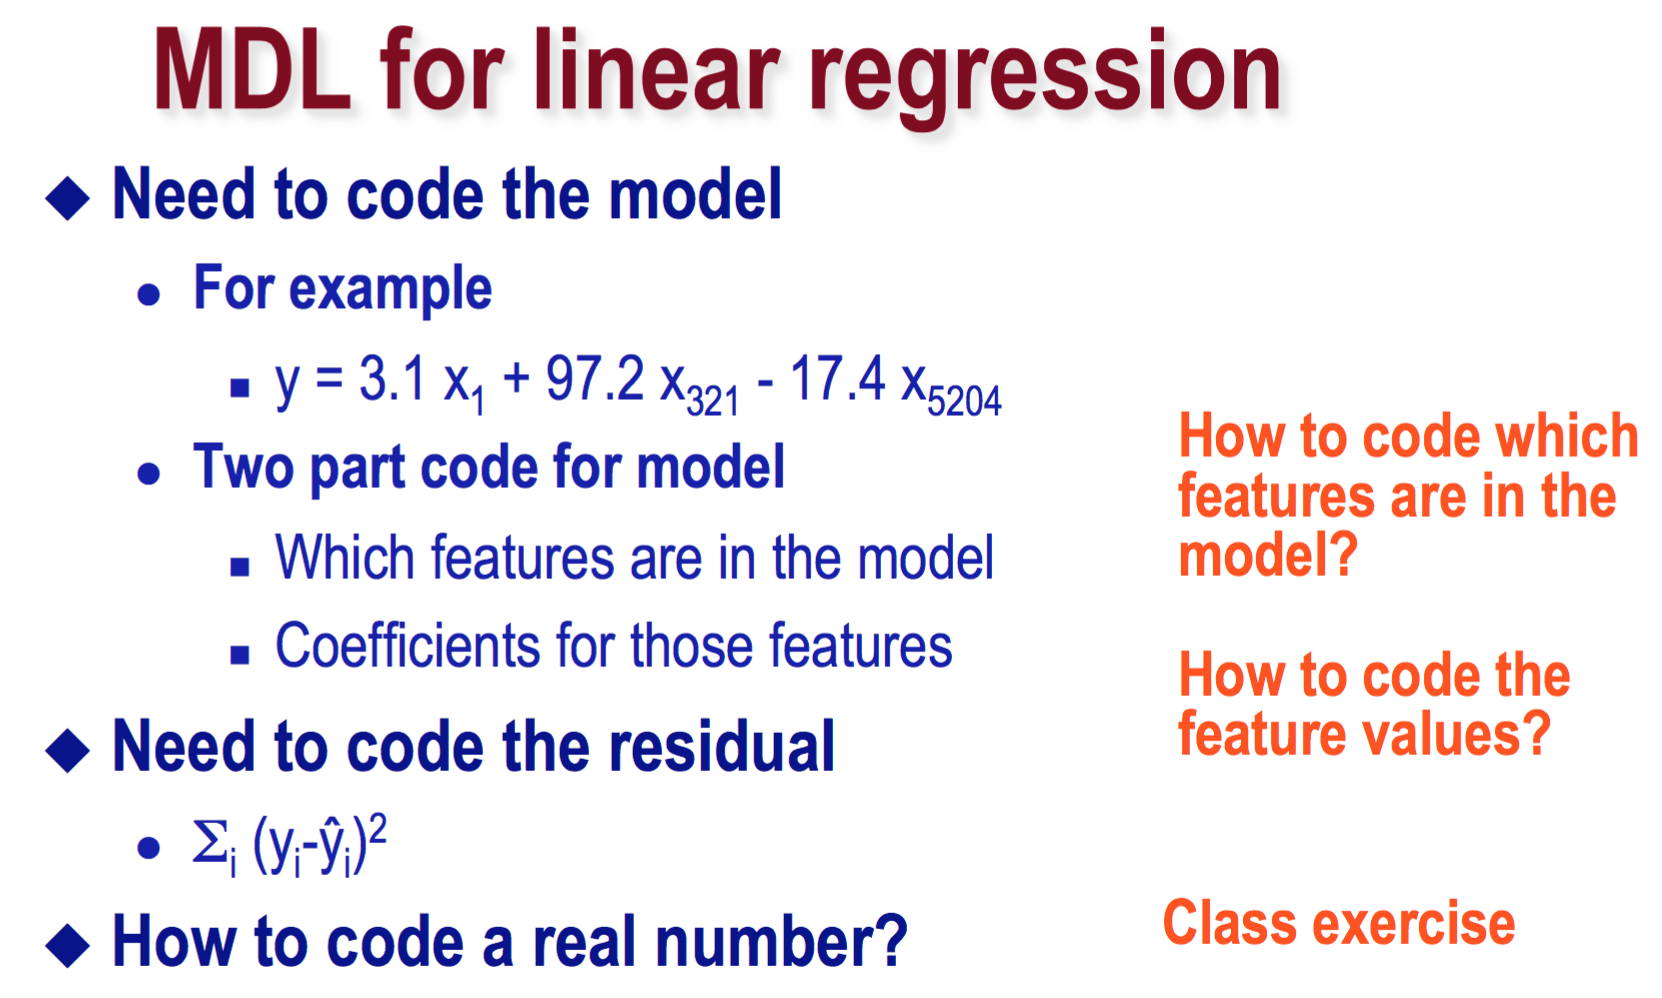
\includegraphics[width=2.5in]{mdl_1.png}
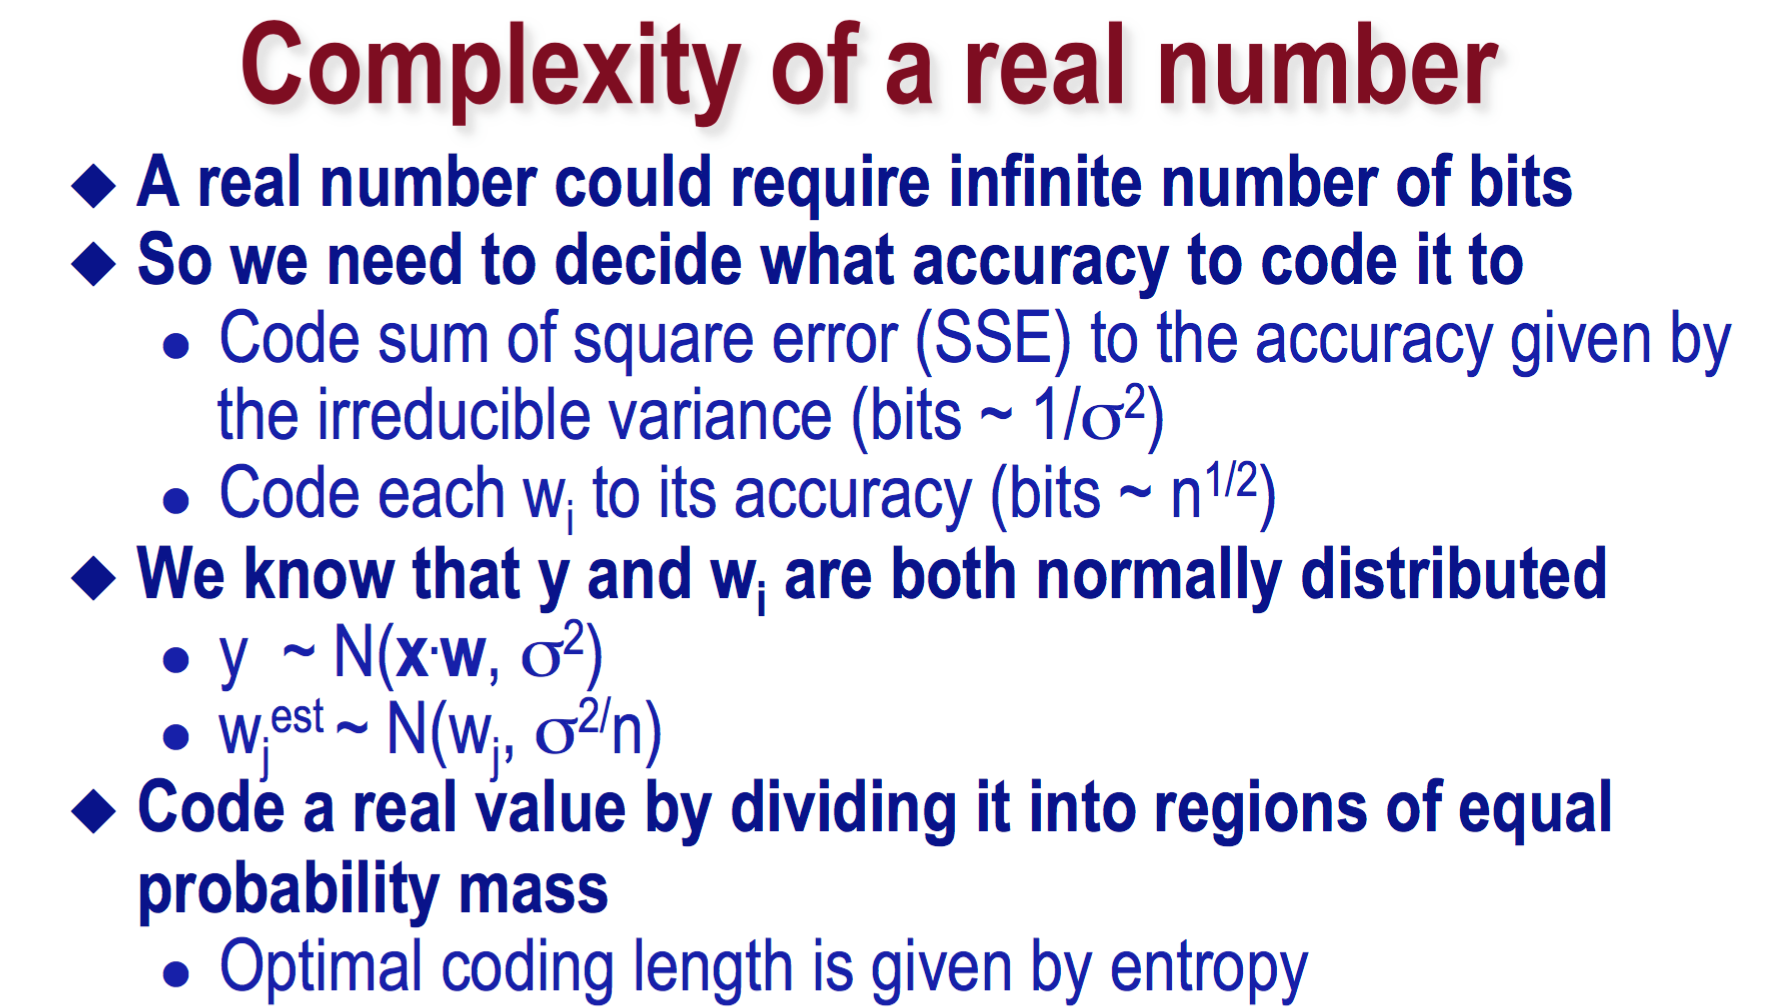
\includegraphics[width=2.5in]{mdl_2.png}
\end{figure}

\subsection{MDL linear regression}

\textbf{Code the residual/data log-likelihood}
\begin{align*}
\log(\text{likelihood}) = n\log(\sqrt{2\pi}\sigma) + \frac{1}{2\sigma^2}\exp(-\lVert y-\hat{y} \rVert)_2^2
\end{align*}

\textbf{Code the model}
\begin{itemize}
\item For each feature, is it in the model?
\item If it is included, what is its coefficient?
\end{itemize}

Choosing models to code the residuals and model \textbf{is exactly} the bias, variance tradeoff!! If we fit a super complex data, need less bits to code residual (smaller bias) but variance will be higher so need more to code the model. If we fit a super simple mode, need more bits to code residual (larger bias) but variance will be smaller so need less to code the model.\\
\\

\textbf{But we don't know $\sigma^2$}, the irreducible error
\begin{itemize}
\item Option 1 - use estimate from previous iteration ;
\begin{equation*} \sigma^2 = \text{Err}_{q-1} \end{equation*}
\item Option 2- use estimate from current iteration ;
\begin{equation*} \sigma^2 = \text{Err}_{q} \end{equation*}
\end{itemize}

\subsection{Complexity of features}

If you expect q features in the model, each will come in with probability $\frac{q}{p}$ (p total features under consideration). The total cost \textbf{for all p features} is then
\begin{equation*} p (-(q/p)\log(q/p) - ((p-q)/q)\log((p-q)/p)) \end{equation*}
Note: we multiply by p at the beginning because we the total cost is for all $p$ features, so pay for all of them. $-(q/p)\log(q/p)$ is for features in the model and $(p-q)/q)\log((p-q)/p)$ is for features not in the model. \\
\\
Note: complexity of model increases logarithmically with number of features. AND THIS COSTS US IN BITS! To make it worth it we must also be lowering number of bits needed to code residaul (ie. lower bias) 

\begin{ex}
\begin{itemize}
\item If $\frac{q}{p}=\frac{1}{2}$, total cost is p ; $cost/feature = 2 bits$
\item If $\frac{q}{p}=1$, total cost is $\log(p)$ ; $cost/feature = 1 bit$
\end{itemize}
\end{ex}

\textbf{Regression Penalty Methods}
Minimize $\frac{\text{Err}_q}{2\sigma^2} + \lambda \lVert \beta \rVert_0$ ($L_0$ penalty on coefficients, SSE with the $\lVert \beta \rVert_0=q$ features) 

\begin{table}[H]
\centering
\caption{My caption}
\label{my-label}
\begin{tabular}{l|l|l}
Method & Penalty &  \\
\hline
AIC    & 1       & code coefficient using 1 bit  \\
BIC    & $(1/2)\log(n)$ & code coefficient using $n^{1/2}$ bits \\
RIC    &  $\log(p)$ & code feature presence/absence; prior:one feature will come in 
\end{tabular}
\end{table}

AIC is too cheap!! It will probably overfit and add too many features (but if you have a ton of features, might be a good bet). When $n>p$ and not too many features, BIC is probably a good bet. Often in ML, we are in RIC land. 

\begin{ex}
\begin{itemize}
\item You expect 10 out of 100,000 features, n=100  - RIC
\item You expect 200 out of 1,000 features, n=1,000,000 - BIC
\item You expect 500 out of 1,000 features, n=1,000 - AIC
\end{itemize}
\end{ex}

\textbf{Why does MDL work?}
\begin{itemize}
\item We want to tune model complexity - how many bits should we use to code the model?
\item Minimize: Test error = training error + penalty = bias + variance
\end{itemize}

\begin{ex}
\begin{itemize}
\item You think 10 out of 100,000 features will be significant - probably use $L_0$ norm with RIC
\item You think 500 out of 1,000 features will be significant - use anything \textbf{but} $L_0$ with RIC
\end{itemize}
\end{ex}

Note: RIC is quite similar to Bonferroni correction. 

\section{Neural Networks}

Uses \textbf{very} flexible model forms : $\hat{y}=f(x;\theta)$. Uses different loss functions such as $L_2$ norm, log-likelihood, logistic/softmax, etc. If we knew the functional form of the data, we wouldn't need such flexible forms used in neural nets!

\begin{itemize}
\item Non-parametric (or technically, semi-parametric) - flexible model form
\item Used when there are vast amounts of data
\end{itemize}

Deep Learning forms:
\begin{itemize}
\item Supervised - convolutional, recurrent  (LSTM) ; generalize logistic reg to semi-parametric form
\item Unsupervised - autoencoder ; generalize PCA to semi-parametric form
\item Semi-supervised
\item Reinforcement Learning
\end{itemize}

Below is a simple three layer artificial neural net (ANN). It basically stacks logistic regressions. 
\begin{figure}[H]
\centering
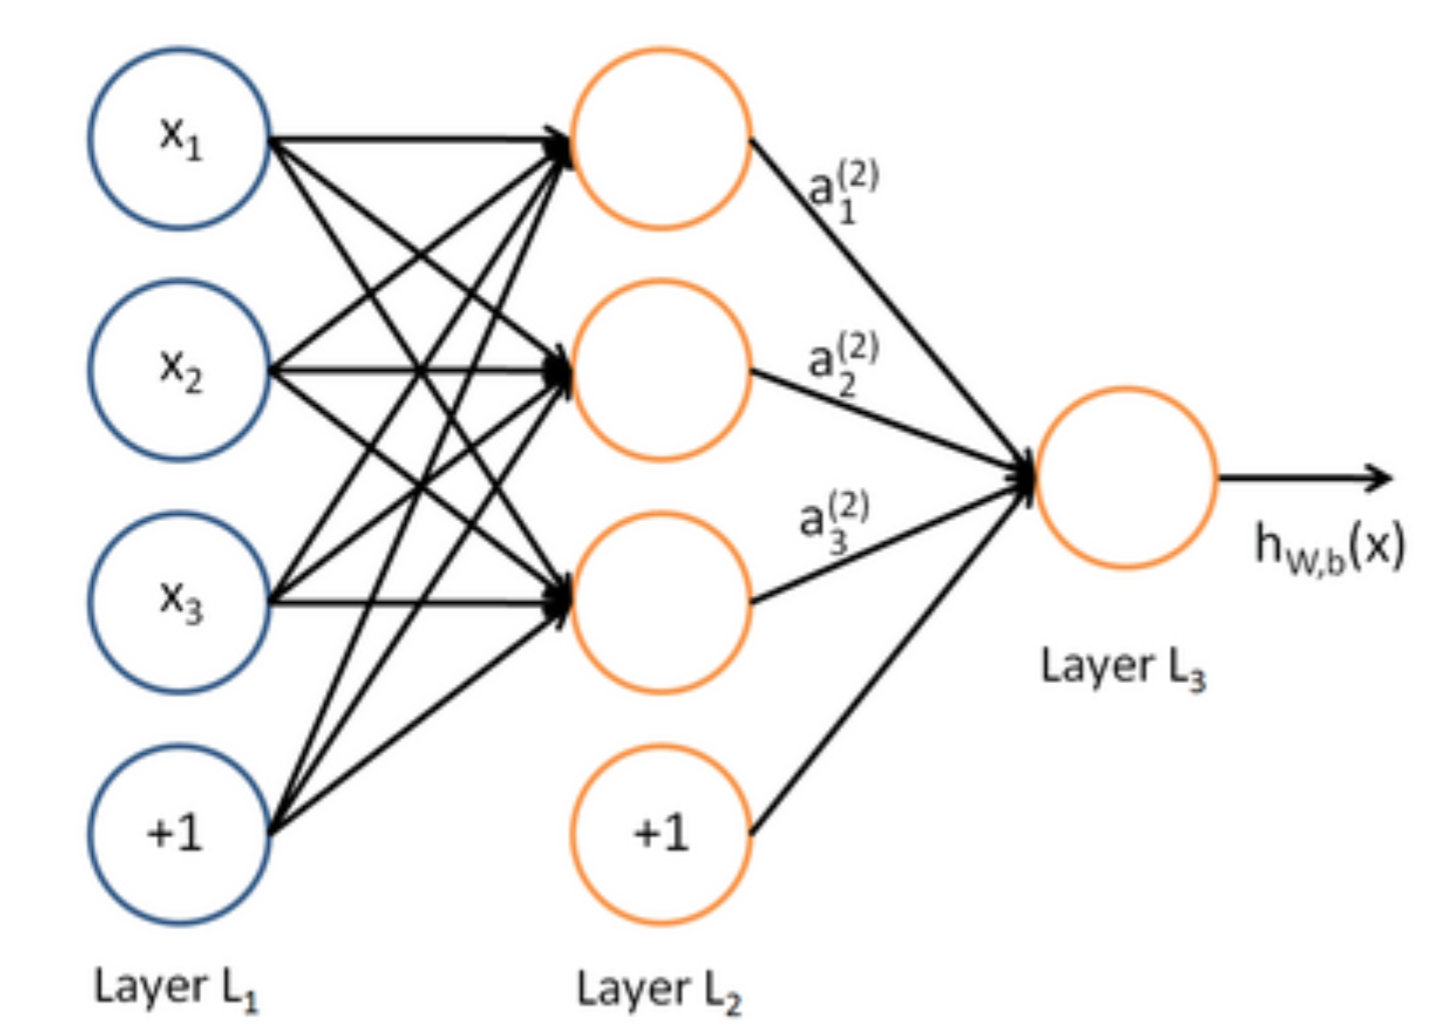
\includegraphics[width=3in]{nn_simp.png}
\end{figure}

Let $\sigma$ be the sigmoid (logistic) function. Then prediction could be something like
\begin{align*}
\hat{y} = \sigma \left[ \sum_{k=1}^3 a_k \sigma \left(\sum_{j,k} w_{j,k}x_j\right)\right]
\end{align*}

Since the above is non-linear, to minimize the loss (for instance $\lVert y-\hat{y}\rVert_2^2$), we use (stochastic) gradient descent to estimate parameters and use the chain rule (backpropagation) to find derivatives. The \textbf{number of parameters} in the model above is given by \emph{each line}, ie number of parameters is number of lines above.\\
\\

Can add more hidden layers (yellow circles) to get a deep network!!
\begin{figure}[H]
\centering
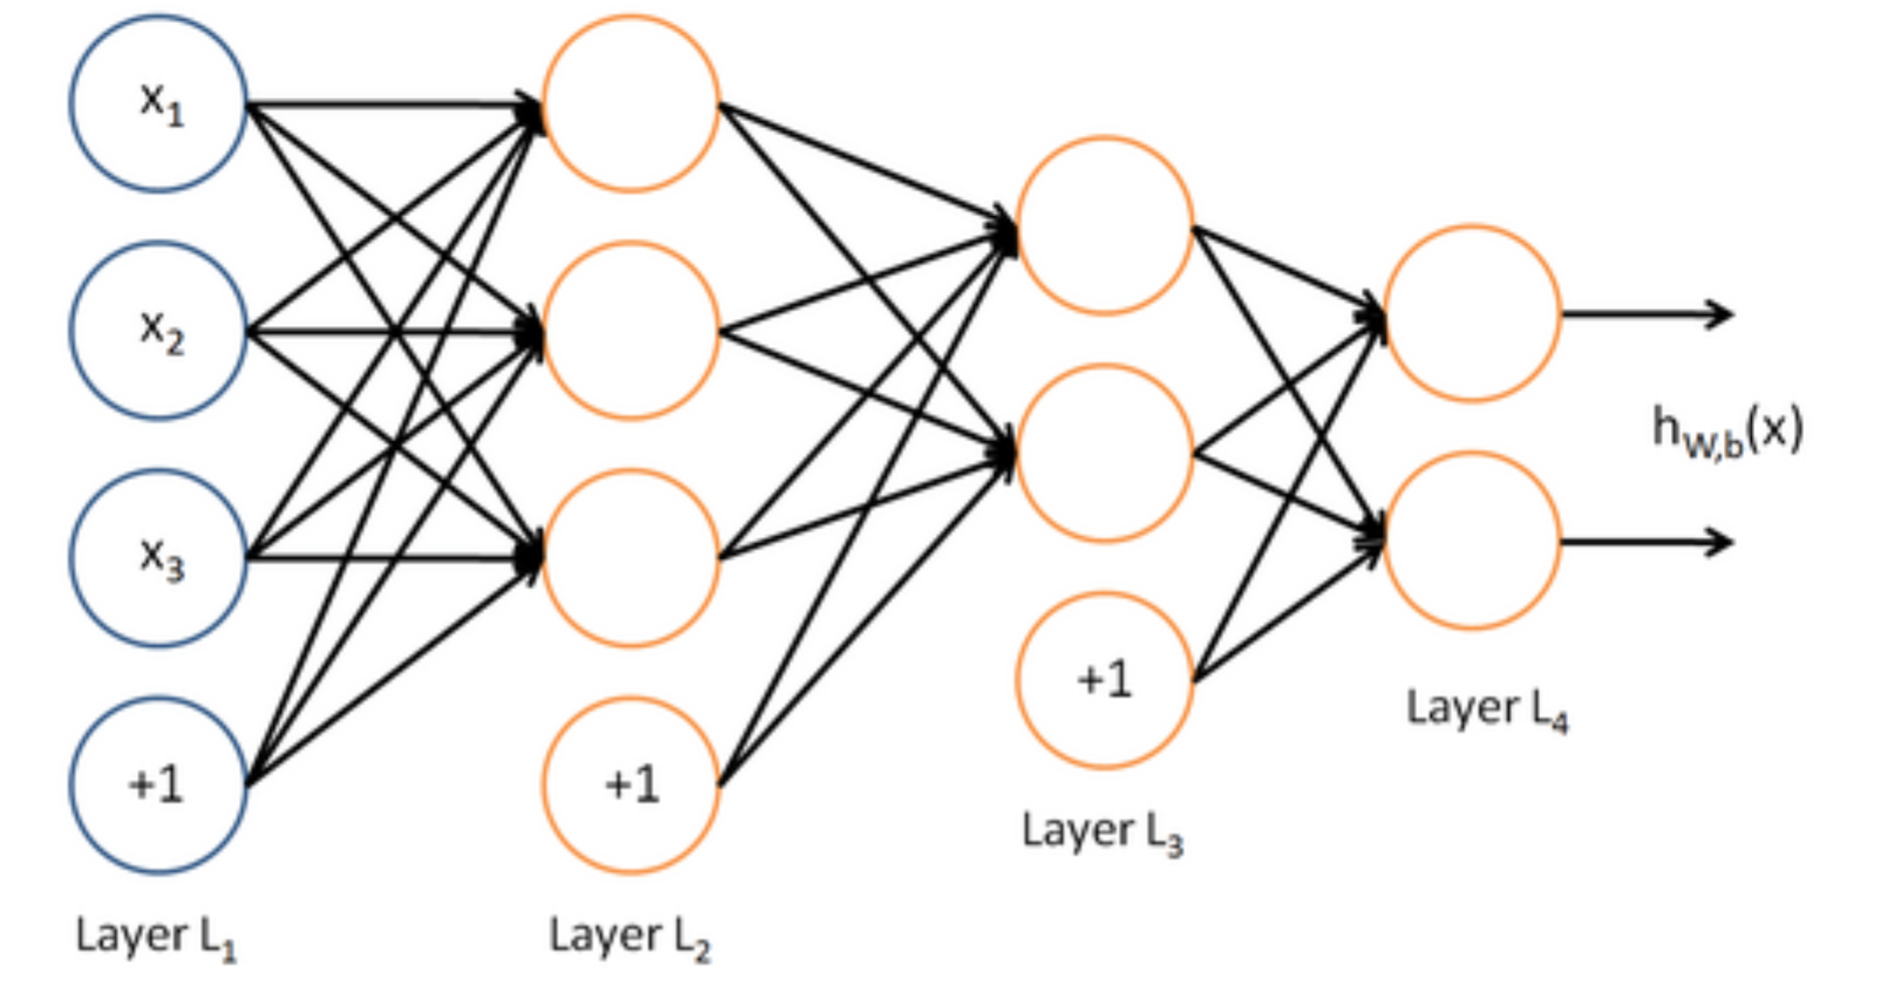
\includegraphics[width=3in]{nn_deep.png}
\end{figure}

The intuition for adding more layers is that each layer is essentially doing feature detection. Each layer automatically determines features that when fed into another layer can predict whatever very well!

\begin{defn}
\textbf{Fully connected network} - each input in layer is connected to the next layer
\end{defn}

ANNs input \textbf{percepts} to output categories or actions
\begin{itemize}
\item Image of object $\rightarrow$ what it is
\item Board position $\rightarrow$ probability of winning
\item Sequence of words in English $\rightarrow$ their Chinese translation
\end{itemize}

Classic, revolutionary paper : ImageNet Classification with Deep Convolutional Neural Networks \\
\\
\textbf{Evolution of functions}:
\begin{itemize}
\item Logistic function - traditional, works okay
\item Hyperbolic tangent - very bad, slow to train
\item \textbf{Rectified Linear Unit (ReLU)} - very good, quick to train ; $f(x)=x^+ = \text{max}(0,x)$
\item Can use any nonlinear function
\end{itemize}

\subsection{AlexNet}

\begin{itemize}
\item 7 hidden layers ; 5 convolutional layers and 2 fully connected layers
\item In vision, neuron may only get inputs from limited set of ``nearby" neurons
\item \textbf{Local/Max pooling}: partitions the input image into non-overlapping rectangles and outputs the maximum value for each. Follows 1st, 2nd, and 5th convolutional layers in AlexNet. See example below
\end{itemize}

Taking the max is intuitive because in images, we are often interested in knowing \emph{if} something is there or not. ie. is a cat in the image?

\begin{figure}[H]
\centering
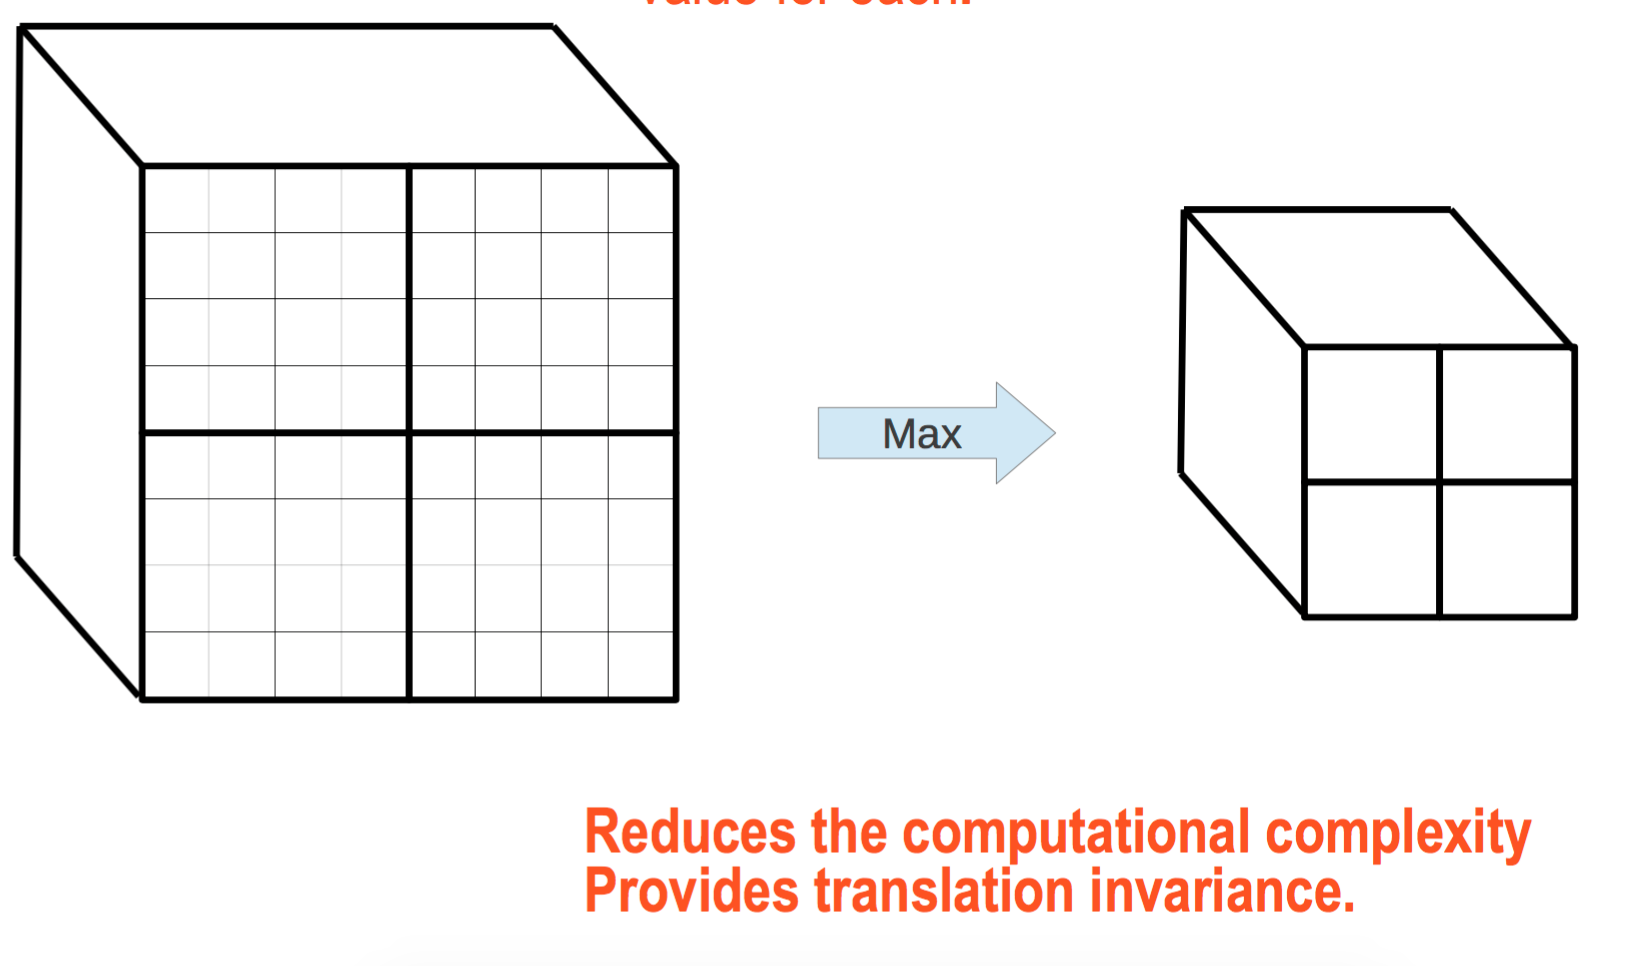
\includegraphics[width=3in]{cnn_pooling.png}
\end{figure}

\textbf{How did AlexNet do?}:
\begin{itemize}
\item 60 million parameters, so overfit A LOT. To combat this, generated pseudodata by shifting images slightly so that they get more examples but dont have to label more data. $\rightarrow$ DATA AUGMENTATION
\item For example, thought tape player was a cellular telephone because in 2012 cell phones were much more frequent
\end{itemize}

\subsection{Modern Deep Nets}

\begin{itemize}
\item Often use ReLUs - less problems of saturation than logistic
\item Use a variety of loss functions - often log likelihood (uses softmax: $P(y=j|x)=\frac{\text{exp}(w_j^Tx)}{\sum_k \text{exp}(w_k^Tx)})$
\item Can be very deep
\item Solved with mini-batch gradient descent
\item Regularized using $L_2$ penalty plus ``dropout"....or partial convergence (form of regularization by stopping early somehow the weights are smaller?)
\end{itemize} 

Note that softmax is often used in the final layer of NNs. Generalization of the logistic function that ``squashes" a K-dim vector of arbitrary real values to a K-dim vector $\sigma(z)$ of values in the range [0,1] that add up to 1. 

\begin{defn}
\textbf{Dropout} 
\begin{enumerate}
\item randomly (temporarily) remove a fraction $p$ (usually 0.5) of the nodes (w/ replacement)
\item Do gradient descent on the other fraction
\item Then repeat
\end{enumerate}
Repeatedly doing this samples (in theory) over exponentially many networks (bounces network out of local minima). For the final network, use all the weights but shrink them by $p$. 
\end{defn}

\subsection{Stochastic Gradient Descent}
With standard gradient descent, we would calculate error over \textbf{all} data points. \textbf{Stochastic gradient descent} does this for each point at a time. Ie. if $Err = \sum_{i=1}^n (y_i-\hat{y}_i)^2$, normal GD would calculate $\frac{dErr}{d\overrightarrow{w}}$, which is over all (for example million) points. Stochastic GD  calculates derivative of $Err_= (y_i-\hat{y}_i)^2$ instead which is much cheaper. \\
\\
\textbf{Properties}:
\begin{itemize}
\item Stochastic GD is probably faster and bouncier - can essentially do ``online" learning by updating weights as each data point comes in 
\item Normal GD has been proven to decrease error each iteration ; not so for stochastic GD bc we are only doing one weight at a time
\item Learning rates are quite different
\item FOR ALL GD stuff we know when convergence is reached by cross-validation.
\end{itemize}

Most software that does GD approximates the derivative of the error using symmetric version (doesn't actually use the chain rule):
\begin{align*}
\frac{dErr(w)}{dw} = \frac{Err(w+h)-Err(w-h)}{2h}
\end{align*}

Note: the above is done for each weight to see how it changes the error. \\
\\
In practice, nobody uses either!!! Normal GD is too slow and stochastic GD is too bouncy. They use \textbf{minibatch} GD. 
\begin{defn}
\textbf{Mini-Batch GD}: does GD batch by batch (ie. 20 points at a time). Much faster and more stable than either of the above. Mini-Batch GD has stochastic GD and normal GD as special cases (batch=1 or batch=n)
\end{defn}

\begin{defn} \textbf{Momentum}:
\begin{align*}
\Delta w^t = \eta \frac{dErr}{dw} + m \Delta w^{t-1}
\end{align*}
Want the hessian, but this is a compromise
\end{defn}

\subsection{Learning Rate}

\begin{itemize}
\item Want to adjust the learning rate over time, ie. make the learning rate smaller as we get closer to local max
\begin{align*} \Delta w^t = \eta(t) \frac{dErr}{dw} \end{align*}
\item Could also have different learning rate for each weight - \textbf{Adagrad}: makes the learning rate depend on previous changes in each weight. Increases the learning reate for more sparse parameters and decreases the learning rate for more sparse ones. 
\begin{align*}
\Delta w_j^t = \frac{\eta}{\lVert \delta w_j^{\tau}\rVert_2}\frac{dErr}{dw_j}
\end{align*}

\end{itemize}




\end{document}
